\documentclass[10pt,twocolumn,letterpaper]{article}

\usepackage{cvpr}
\usepackage{times}
\usepackage{epsfig}
\usepackage{graphicx}
\usepackage{amsmath}
\usepackage{amssymb}
\usepackage{overpic}
\usepackage[dvipsnames]{xcolor}
\definecolor{accent}{RGB}{179,81,109}

\usepackage[pagebackref=true,breaklinks=true,letterpaper=true,colorlinks,bookmarks=false]{hyperref}

\def\cvprPaperID{****} 
\def\httilde{\mbox{\tt\raisebox{-.5ex}{\symbol{126}}}}

\ifcvprfinal\pagestyle{empty}\fi
\begin{document}

\title{\LaTeX\ Author Guidelines for CVPR Proceedings}

\author{First Author\\
Institution1\\
Institution1 address\\
{\tt\small firstauthor@i1.org}
\and
Second Author\\
Institution2\\
First line of institution2 address\\
{\tt\small secondauthor@i2.org}
}

\maketitle


\begin{abstract}
   The ABSTRACT is to be in fully-justified italicized text, at the top
   of the left-hand column, below the author and affiliation
   information. Use the word ``Abstract'' as the title, in 12-point
   Times, boldface type, centered relative to the column, initially
   capitalized. The abstract is to be in 10-point, single-spaced type.
   Leave two blank lines after the Abstract, then begin the main text.
   Look at previous CVPR abstracts to get a feel for style and length.
\end{abstract}

\section{Settings}
A hand in motion can be described by two types of parameters.
\begin{itemize}
\item Pose parameters \textit{(joint angles and rigid rotation and translation of the hand)} $\theta \in \mathbb{R}^{N_{\theta}}$ change with time. 
\item Shape parameters \textit{(length and thickness of fingers phalanges, position of finger bases, shape of the palm)} $\beta \in \mathbb{R}^{N_{\beta}}$ vary between different people while staying constant for each person. 
\end{itemize}
Given a sequence of depth sensor images $\mathcal{D}_n$, the goal of our system is to get best possible estimate of shape parameters $\hat{\beta}_n$ from the input available so far.

How much information do we need to have a good guess of $\beta$? A trivial lower bound would finding $\beta$ from a single sensor image. This scenario could be conceived for palm shape and fingers thickness, since they are ``visible'' in any hand pose. However, the phalanges length cannot be estimated when the fingers are straight; moreover the locations of finger bases are hidden under the skin and can only be inferred after seeing a range of hand poses. Sensor noise and $2,5 D$ nature of the data further aggravate the problem. 
Previous authors \cite{joseph2016fits} and \cite{tkach2016sphere} suggested to find hand shape from a set of manually picked hand poses. 

\textbf{Advantages of online optimization over batch optimization}
\begin{itemize}
\item \textit{user experience:} the user does not have to track with uncalibrated model first, manually pick the poses, wait till batch optimization finishes; also there is an immediate feedback on the result quality, so no need for several ``blind'' trials.
\vspace{-1em}
\item \textit{system efficiency:} there is not need to solve a potentially very big linear system, thus hand tracking algorithm will use less computational resources; potentially it can run on a lighter hardware.
\item \textit{result quality:} this claim will be /*hopefully*/ proven experimentally. 

\begin{itemize}
\vspace{-1em}
\item By default performance of batch algorithm is an upper bound for online algorithm running on the same data. However, in practice online algorithm can use any amount of data and batch algorithm is limited by the available memory and computational power.
\item  Also, it is important that to take into account that the problem is solved with local optimization. If each frame of batch optimization is initialized far away from the true hand parameters, the solver can get stack in bad local optimum. (Shape prior should help in this case, but a good prior is difficult to learn). Online optimization, if it works properly, can have better and better initialization with every frame.
\end{itemize}
\end{itemize}

\subsection {Hand Model}

\begin{figure}[h!]
\centering
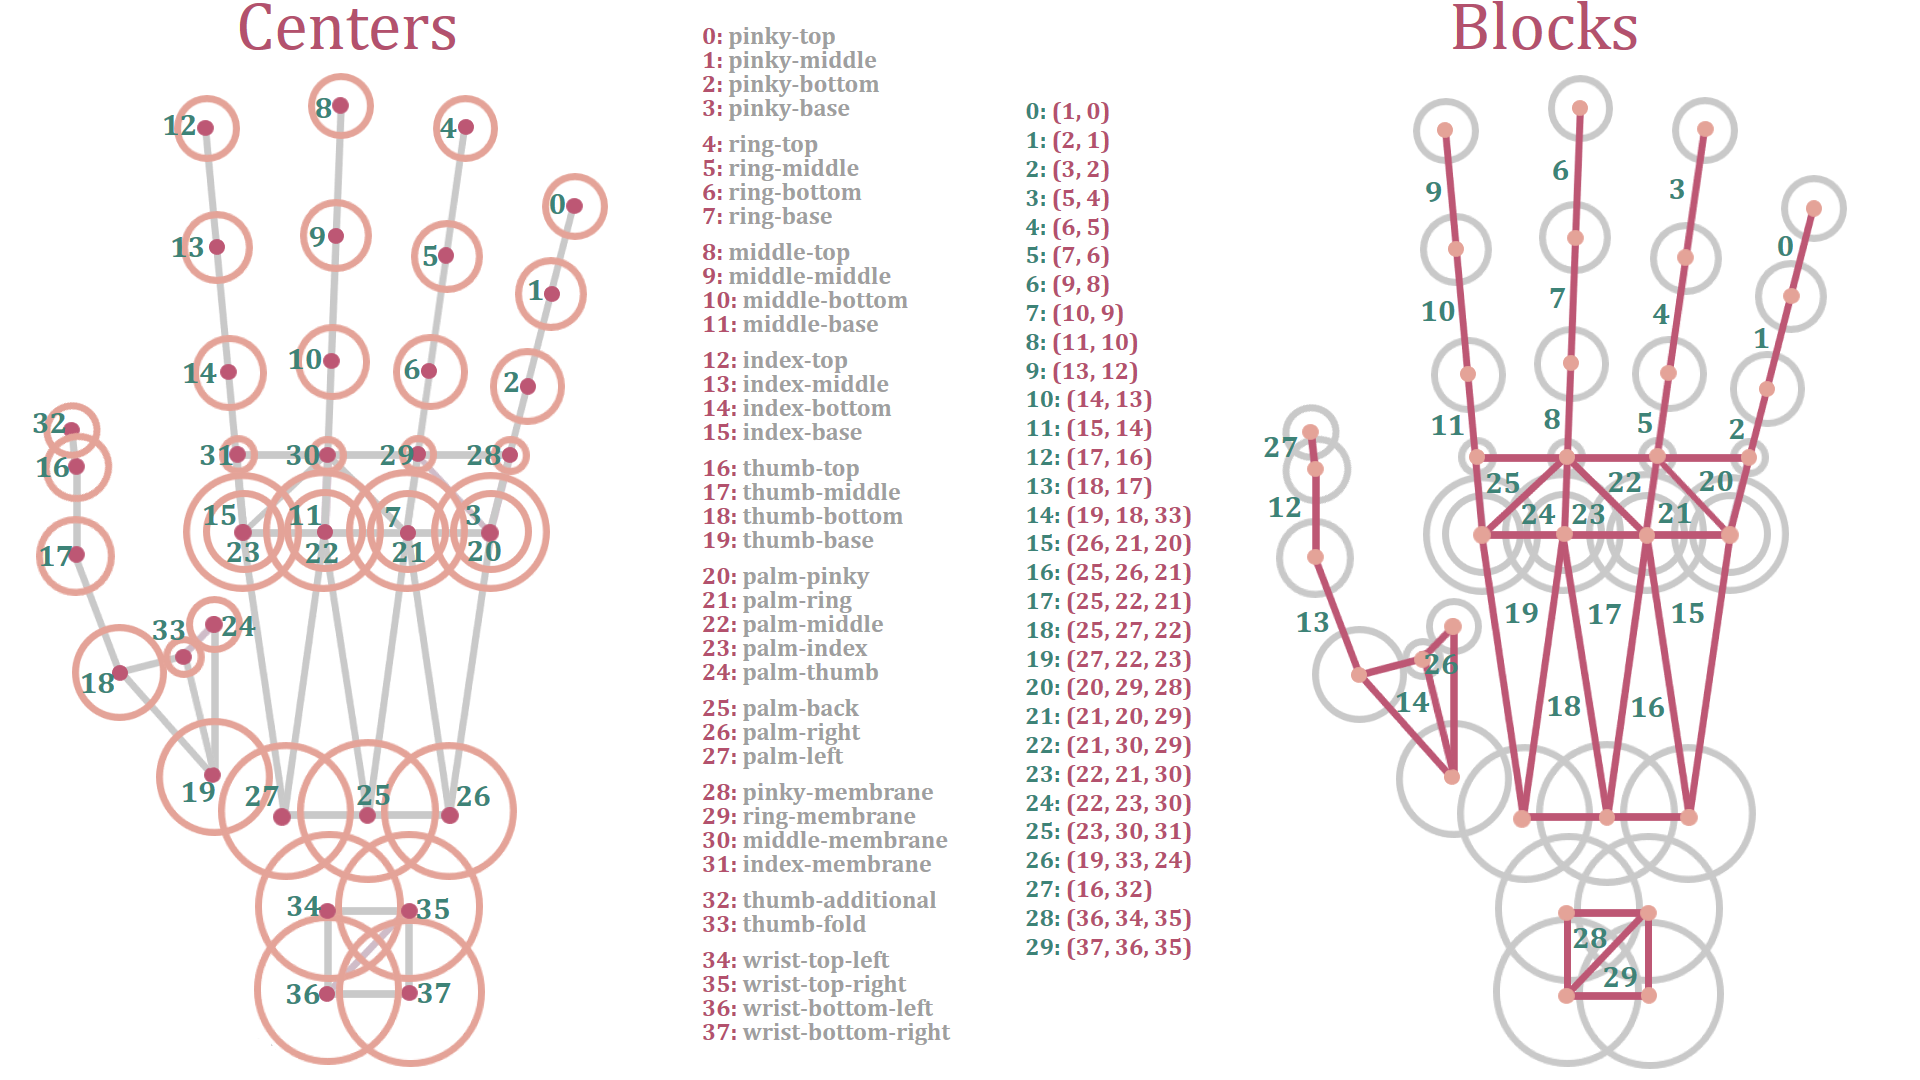
\includegraphics[width=1\linewidth]{figures/centers-blocks}
\caption{Sphere-mesh representation}
\label{fig:centers-blocks}
\end{figure}

\begin{figure}[h!]
\centering
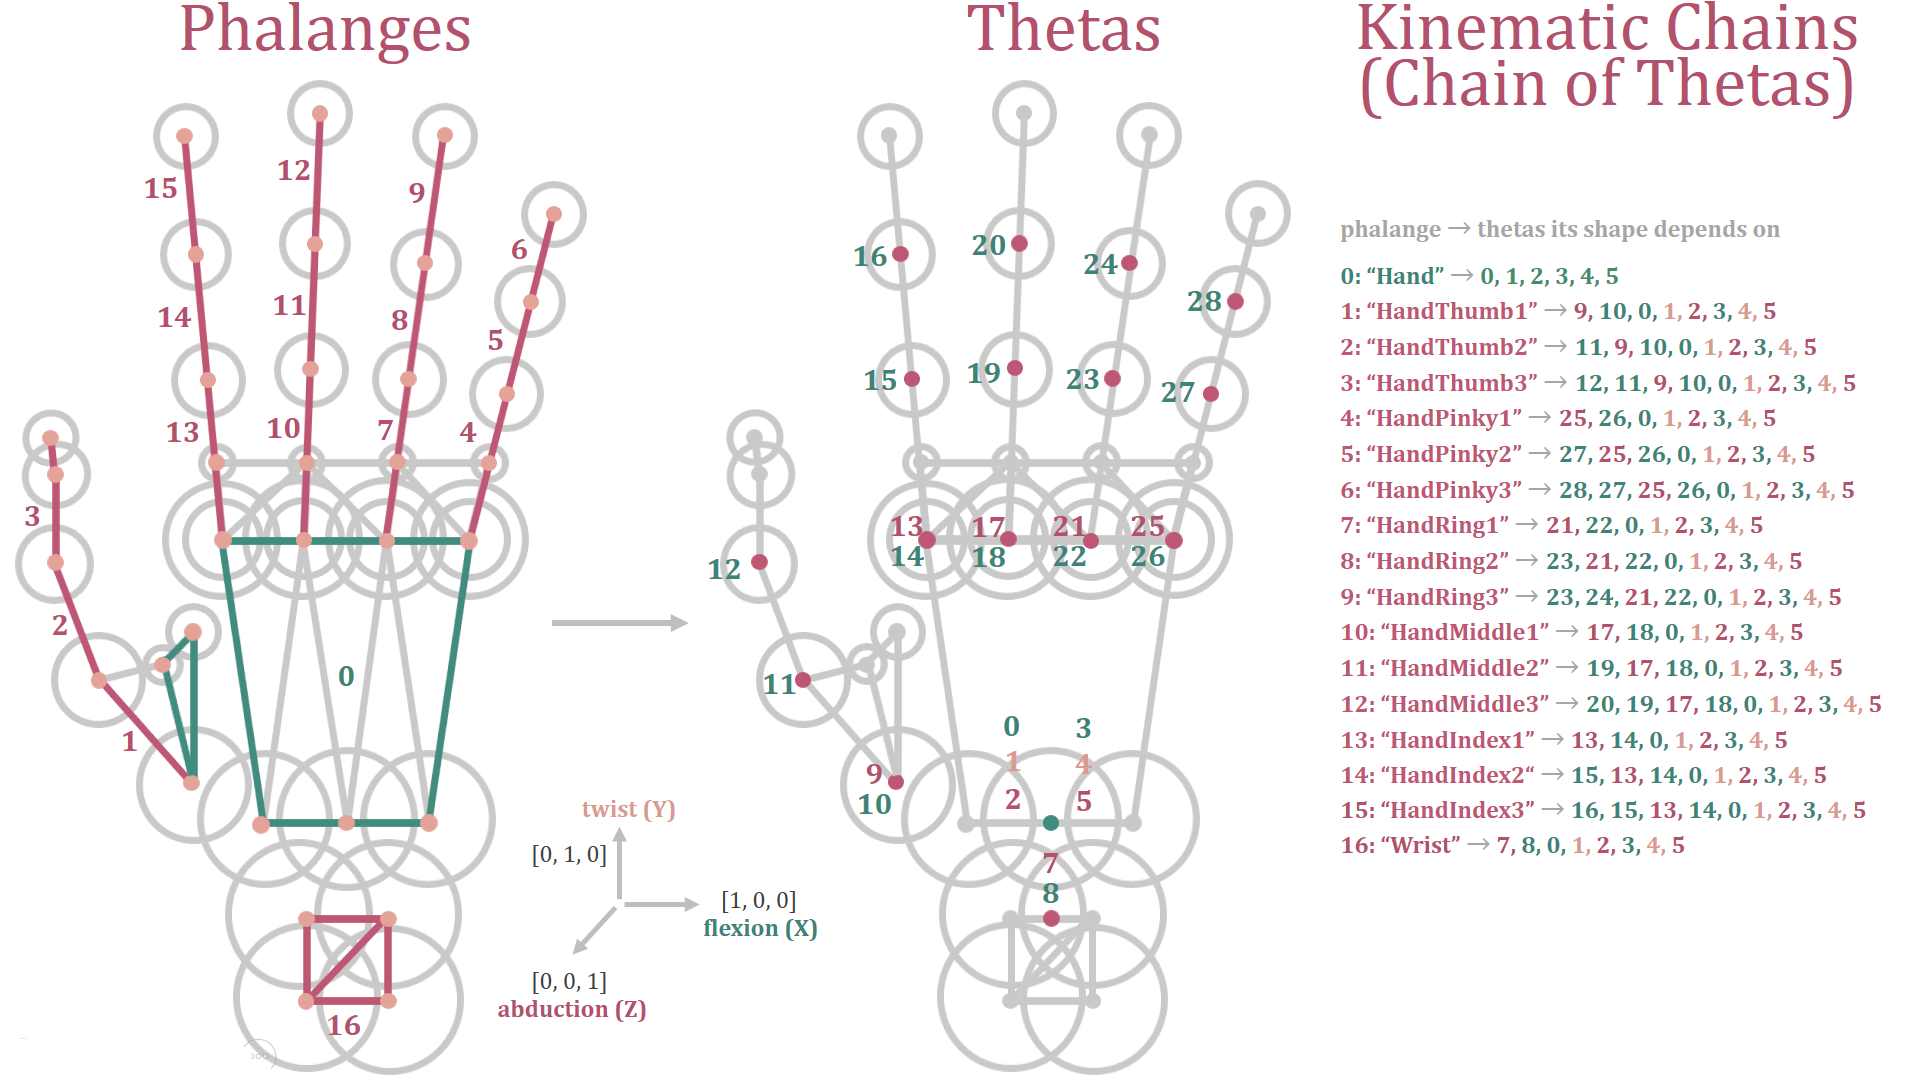
\includegraphics[width=1\linewidth]{figures/thetas}
\caption{Pose parameters $\theta$}
\label{fig:thetas}
\end{figure}

\begin{figure}[h!]
\centering
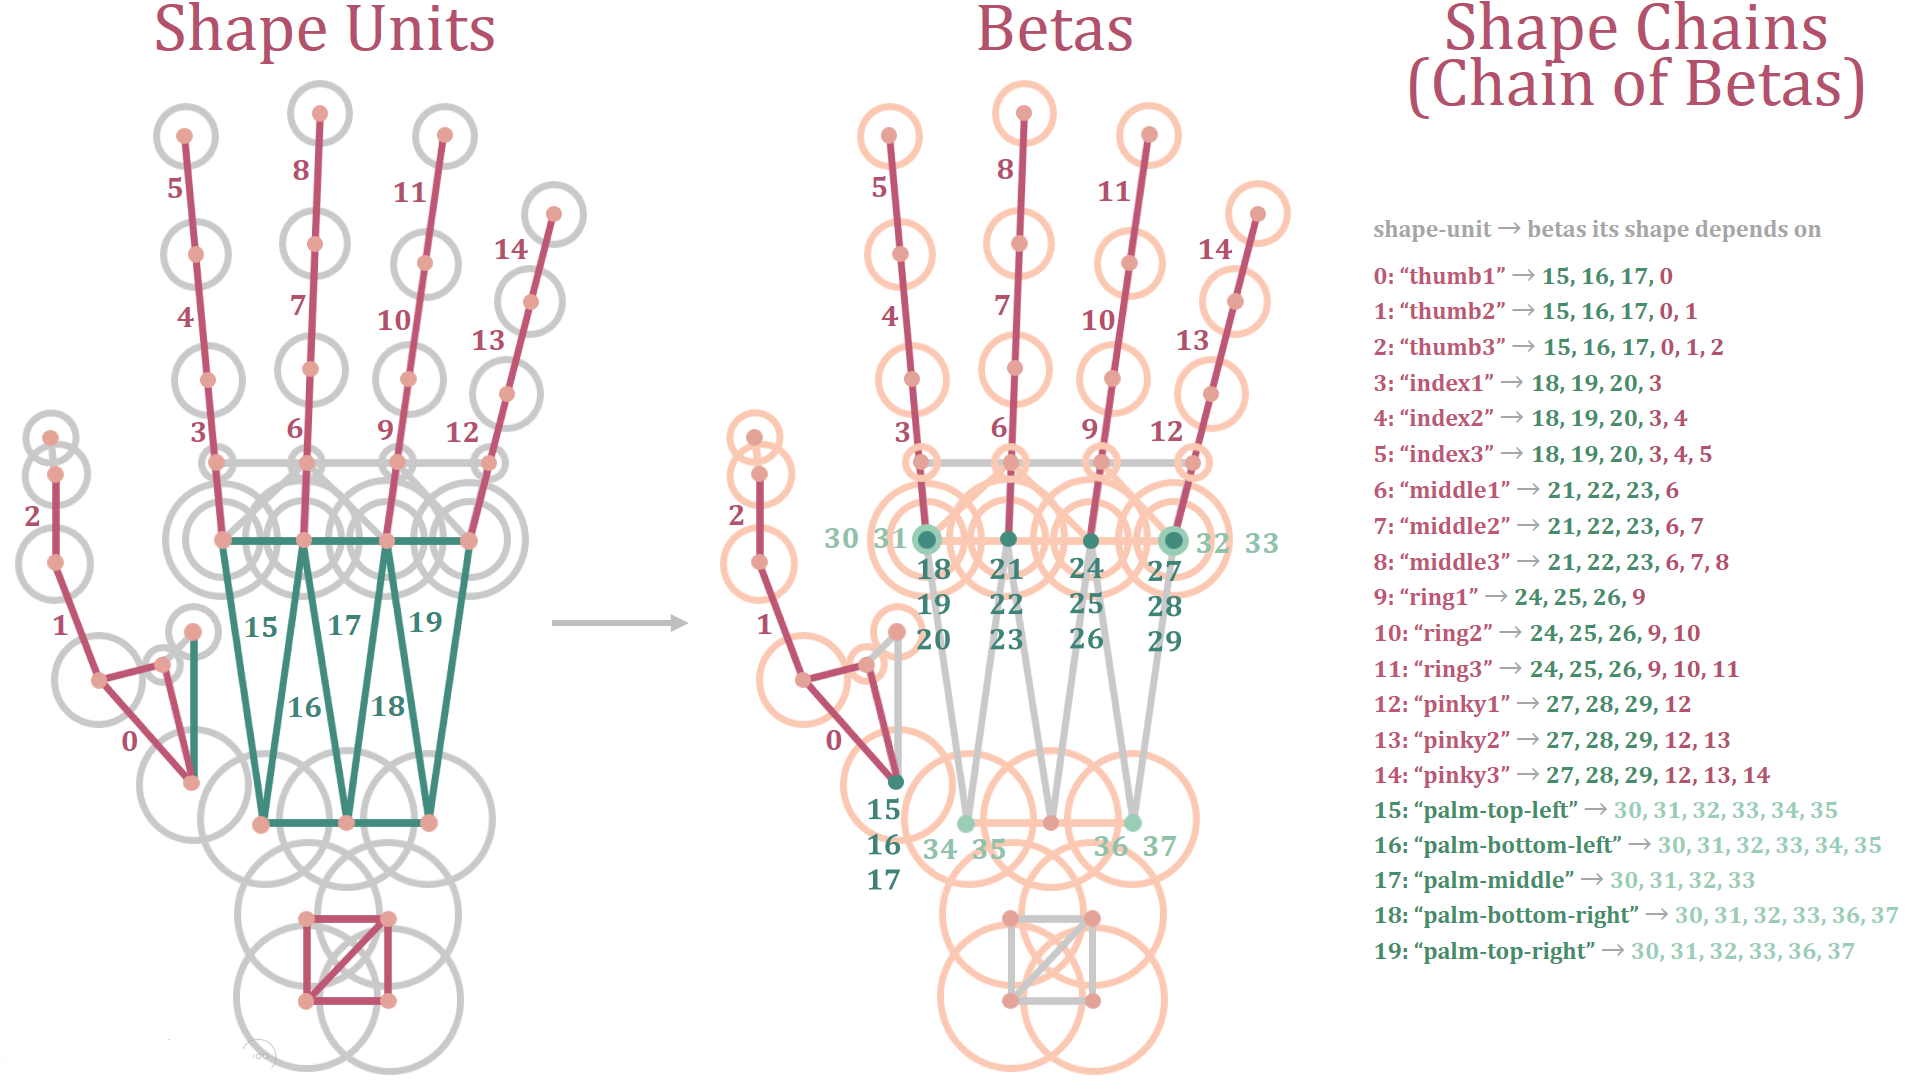
\includegraphics[width=1\linewidth]{figures/betas}
\caption{Shape parameters $\beta$}
\label{fig:betas}
\end{figure}

We use sphere-mesh hand model presented in \cite{tkach2016sphere}, which is a special case of a convolution surface. \textbf{\color{accent}{Maybe briefly recap advantages of sphere-meshes hand model representation}}. 

The skeleton $\mathcal{S} = \{\mathcal{V}, \mathcal{E}, \mathcal{F}\}$ of the sphere-mesh is a planar graph with a fixed topology. Each vertex $\mathcal{V}_i$ corresponds to a sphere with center $c_i \in \mathbb{R}^3$ and radius $r_i \in \mathbb{R}^+$. The radii at intermediate points are given by linear interpolation of the radii at the vertices.
While the skeleton topology is predefined for the class of object ``human hand'', changing centers and radii spans the pose and shape space of human hands.

Note that shape parameters $\beta$ stay constant for a given person and play a different semantic role from pose parameters $\theta$, thus it is helpful to distinguish between to two types of the parameters. Also, it is important to prohibit the degrees of freedom that are not available to the human hand. Thus we use the two representations interchangeably - sphere-meshes representation for closest point correspondences and for rendering and ``semantic'' representation for finding $\beta$ and $\theta$.
The centers $c_i$ are computed from $\beta$ and $\theta$ using forward kinematics with $\beta$ being transitional degrees of freedom and $\theta$ - rotational degrees of freedom. The ``impossible'' degrees of freedom are eliminated by only allowing only biologically plausible rotational DOFs at the joints.

\subsection {Parametrization}

A point on the model surface $m_i$ is defined by its barycentric coordinates $\{\kappa_1, \kappa_2, \kappa_3\} $ of its projection $s_i$ on the corresponding skeleton face $\mathcal{F}_j = \{c_{j1}, {c_j}_2, {c_j}_3\}$ and the offset direction $o_i \in \mathbb{R}^3$

\begin{equation}
o_i = G_j^{-1} \frac{m_i - s_i} {\| m_i - s_i \|_2^2}
\end{equation}

where $G_j$ is global transformation of the face $F_j$ given by forward kinematics.

Given the new parameters $\{ \beta', \theta' \}$, the new position of the point is
\begin{align}
\begin{split}
m_i'(\beta', \theta') = \kappa_1 c_{j1}' + \kappa_2 c_{j1}' + \kappa_3 c_{j3}' + \\
 + \;  G_j'(\kappa_1 r_{j1}' + \kappa_2 r_{j2}' + \kappa_3 r_{j3}') o_i
\end{split}
\end{align}

with $c_{j1}' = c_{j1}'(\beta', \theta')$,  $r_{j1}' = r_{j1}'(\beta', \theta')$, $G_j' =G_j'(\theta')$.

\subsection {Independent Solve} \label{sec:independent-solve}

Denote the vector of all hand parameters as $x_n = [\theta_n; \beta_n]$ and the segmented hand point cloud in vectorized form as $d_n$. 

Given $d_n$ and initialization of hand pose from previous frame $x_n^0 = x_{n - 1}^*$ we find an independent estimate of $x_n^*$ by local Levenberg-Marquardt optimization of an objective similar to \cite{tkach2016sphere}

\begin{equation}
x_n^* = \operatorname{argmin}_{x_n} \sum_{\tau \in \mathcal{T}} E_{\tau}(d_n, x_n) \label{eq:energies}
\end{equation}

where the energy terms in the objective function are the following:

\begin{itemize}
\item \textbf{d2m} model should be close to data
\vspace{-1em}
\item \textbf{m2d} data should be close to model
\vspace{-1em}
\item \textbf{limits} joint limits should hold
\vspace{-1em}
\item \textbf{collision} fingers should not interpenetrate
\vspace{-1em}
\item \textbf{shape} model shape should be plausible
\vspace{-1em}
\item \textbf{pose} model pose should be plausible
\end{itemize}

See \cite{tkach2016sphere} for more details about energy terms. \textbf{\color{accent} Explain shape term somewhere later.}

\subsection {Posterior distribution of the parameters} \label{sec:posterior}

All the energy term $E_{\tau}(d_n, x_n)$ can be rewritten in a form $\|I_{\tau} d_n - F_{\tau} (x_n)\|_2^2$ with $I_{d2m}$ an identity matrix, $I_{m2d}$ a permutation(/reduction?) matrix that removes from $d_n$ the entries that are not the closest for any model point and the remaining $I_{\tau}$ all zeros matrices. 
Denote $\left[F_{d2m}^T(x_n), ..., F_{pose}^T(x_n)\right]^T$ as $F(x_n)$ and overload $d_n$ as  $\left[(I_{d2m} d_n)^T, ..., (I_{pose} d_n)^T\right]^T$  for brevity of notation.

Given the hand point cloud at the first frame $d_1$, we find the best-fitting parameters (see Section \ref{sec:independent-solve})

\begin{equation}
x^*_1 = \operatorname{argmin}_{x_1} \underbrace{\log  P(d_1|x_1)}_{L(x_1)} \label{eq:independent}
\end{equation}

with $P(d_1|x_1) = \exp \left( - (d_1 - F(x_1))^T (d_1 - F(x_1)) \right)$.

Expanding the log-likelihood of the data $L(x_1)$ around $x_1^*$ we get
\begin{align}
\begin{split}
 L(x_1) \approx L(x_1^*) + \underbrace{\frac{\partial L}{\partial x_1}(x_1^*)}_{= 0 \text{ at extremum}}(x_1 - x_1^*) - \\
- 0.5(x_1 - x_1^*)^T \underbrace{\frac{\partial \partial L}{\partial x_1 \partial x_1}(x_1^*) }_{\text{positive definite}}  (x_1 - x_1^*) \\
\end{split}
\end{align}

with $\frac{\partial L}{\partial x_1}(x_1^*) = - 2 F(x_1^*)^T + 2 F(x_1)^T \frac{\partial F}{\partial x_1}(x_1^*)  $ and 
$\frac{\partial \partial L}{\partial x_1 \partial x_1}(x_1^*) = 2  \frac{\partial F}{\partial x_1}(x_1^*)^T  \frac{\partial F}{\partial x_1}(x_1^*) + 2 F(x_1^*)^T  \frac{\partial \partial F}{\partial \partial x_1}(x_1^*)  \approx  \frac{\partial F}{\partial x_1}(x_1^*)^T  \frac{\partial F}{\partial x_1}(x_1^*)$. Denoting $\frac{\partial \partial L^{-1}}{\partial x_n \partial x_n}(x_n^*) $ as $\Sigma_n$ and taking an exponential of both sides gives:
\vspace{-2em}

\begin{equation}
P(d_1|x_1) \propto \exp\left(- 0.5(x_1 - x_1^*)^T \Sigma_1^{-1}  (x_1 - x_1^*) \right)\\
\end{equation}

Thus, after processing the information from the first frame $d_1$, the quadratic approximation of posterior distribution of hand parameters is a normal distribution $\mathcal{N}\left(\hat{x}_1 = x_1^*,  \hat{\Sigma}_1 = \Sigma_1 \right)$ [ADD REFERENCE].

\subsection {Combining independent measurements} \label{sec:combining}

\textbf{\color{accent}The shape prior should only be used in the first frame, because afterwards it will be incorporated inside of Kalman prior}.

Given the second frame $d_2$, we compute the corresponding value of the parameters $x_2^*$ and their variance $\Sigma_2$ the same way as in \ref{sec:posterior}. The posterior distribution of the parameters now has the form 

\begin{equation}
\mathcal{N}(\hat{x}_2, \hat{\Sigma}_2) = \mathcal{N}(\hat{x}_1, \hat{\Sigma}_1) \mathcal{N}(x_2^*, \Sigma_2)
\end{equation}

Applying the product of Gaussians rule presented in \cite{petersen2008matrix}, we get 
\begin{align}
\begin{split}
\hat{x}_2 = \Sigma_2 (\hat{\Sigma}_1 + \Sigma_2)^{-1} \hat{x}_1 + 
\hat{\Sigma}_1 (\hat{\Sigma}_1 + \Sigma_2)^{-1} x_2^*\\
\hat{\Sigma}_2 = \hat{\Sigma}_1 (\hat{\Sigma}_1 + \Sigma_2)^{-1} \Sigma_2
\end{split} \label{eq:gaussians-product}
\end{align}

In Appendix \ref{app:kalman} it is shown that the Equations \ref{eq:gaussians-product} are equivalent to Kalman filter update with measurement $x_n^*$ and measurement noise covariance $\Sigma_n$. This is important, because, according to P. Maybeck \cite{maybeck1979stochastic}, under the assumptions presented in Appendix \ref{app:kalman} ''... the Kalman filter can be shown to be the best filter of any conceivable form. It incorporates all information that can be provided to it. ''

%%%%%%%%%%%%%%%%%%%%%%%%%%%%%%%%%%%%%%%%%%%%
\begin{table}[!h] 
\centering
\caption{KF: Combining independent measurements\label{tab:kf-like}} 
\begin{tabular}{|c|}
\hline
$x_n^* = \operatorname{argmax}_{x_n} \log P(d_n|x_n)$ \\
$\hat{x}_n = \operatorname{argmax}_{x_n} \underbrace{\log \left( P(x_n|x_n^*) P(x_n |\hat{x}_{n - 1}) \right)}_{L(x_n)}$\\
with \\
$P(x_n |x_n^*) = \exp \left( - (x_n - x_n^* )^T \Sigma_n^{-1}(x_n - x_n^* )\right)$ \\
$P(x_n |\hat{x}_{n - 1}) = \exp \left( - (x_n - \hat{x}_{n - 1} )^T \hat{\Sigma}_{n - 1}^{-1} (x_n - \hat{x}_{n - 1} )\right)$ \\	

$\hat{\Sigma}_n^{-1} = \frac{\partial \partial L}{\partial x_n \partial x_n}(\hat{x}_n) \approx $ \\
\\
$\left[
	\begin{array}{cc}
		\left(\Sigma_n^{-1}\right)^{1/2} \\
		\left(\hat{\Sigma}_{n - 1}^{-1}\right)^{1/2} \\
	\end{array}
\right]^T 
\left[
	\begin{array}{c}
		\left(\Sigma_n^{-1}\right)^{1/2} \\
		\left(\hat{\Sigma}_{n - 1}^{-1}\right)^{1/2} \\
	\end{array}
\right] = \hat{\Sigma}_{n-1}^{-1}  + \Sigma_{n}^{-1}$ \\

\hline
\end{tabular}
\end{table}
%%%%%%%%%%%%%%%%%%%%%%%%%%%%%%%%%%%%%%%%%%%%

\subsection{Regularizing optimization}

Note that the best-fitting parameters $x_n^*$ for the given the single input frame $d_n$ are computed using local LM optimization. Thus, it is crucial that optimization starts in a sensible region of parameters space. The optimization presented in Table \ref{tab:kf-like} does not provided any information about the current estimate of the parameters $\hat{x}_n$ to the independent solve from Section \ref{sec:independent-solve}. One way to remedy this is include the term $P(x_n |\hat{x}_{n - 1})$ directly in the independent solve.

%%%%%%%%%%%%%%%%%%%%%%%%%%%%%%%%%%%%%%%%%%%%
\begin{table}[!h] 
\centering
\caption{Objective function of IEKF \label{tab:iekf-like}} 
\resizebox{0.48\textwidth}{!}{
\begin{tabular}{|c|}

\hline

$\hat{x}_n = \operatorname{argmax}_{x_n} 
\underbrace{\log \left( P(d_n|x_n) P(x_n |\hat{x}_{n - 1}) \right)}_{L(x_n)}$\\ 
with \\
$P(d_n|x_n) = \exp \left( - (d_n - F(x_n))^T (d_n - F(x_n)) \right)$ \\
$P(x_n |\hat{x}_{n - 1}) = \exp \left( -(x_n - \hat{x}_{n - 1})^T \hat{\Sigma}_{n - 1}^{-1} (x_n - \hat{x}_{n - 1})\right)$ \\
\\
$\hat{\Sigma}_n^{-1} = \frac{\partial \partial L}{\partial x_n \partial x_n}(\hat{x}_n) \approx $ \\
\\
$\left[
	\begin{array}{cc}
		- \frac{\partial F} {\partial x_n} (\hat{x}_n) \\
		\left(\hat{\Sigma}_{n - 1}^{-1}\right)^{1/2} \\
	\end{array}
\right]^T 
\left[
	\begin{array}{c}
		- \frac{\partial F} {\partial x_n} (\hat{x}_n) \\
		\left(\hat{\Sigma}_{n - 1}^{-1}\right)^{1/2} \\
	\end{array}
\right] = $\\
\\
$ = \hat{\Sigma}_{n-1}^{-1} + \frac{\partial F} {\partial x_n} (\hat{x}_n)^T \frac{\partial F} {\partial x_n} (\hat{x}_n) = \hat{\Sigma}_{n-1}^{-1}  + \Sigma_{n}^{-1}$	\\
\hline
\end{tabular}
}
\end{table}

In Appendix \ref{app:ieif-lm} we demonstrate that optimizing the objective function presented in Table \ref{tab:iekf-like} using Levenberg-Marquardt algorithm is equivalent to measurement update of Iterated Extended Kalman Filter.

\subsection{Comparing the two optimizations}
The optimization presented in Table \ref{tab:kf-like} will be used as a baseline. It treats the results of the independent solve $x_n^*$ as a measurement, which, arguably can be considered as the simplest way to maintain an online estimate of the parameters. 
The optimization presented in Table \ref{tab:iekf-like} represents the hand tracking system as an Iterated Extended Kalman Filter. It directly outputs the estimated value of the parameters $\hat{x}_n$, using $d_n$ as a measurement.
%%%%%%%%%%%%%%%%%%%%%%%%%%%%%%%%%%%%%%%%%%%%

 \appendix
\section{Kalman Filter (KF)} 
\label{app:kalman}
Following the notation in~\cite{welch1995introduction}, given the measurement $z_n \in \mathbb{R}^M$, the Kalman Filter (KF) latent state $x_n \in \mathbb{R}^N$ update equations are:
% 
\begin{align}
x_n &= A x_{n - 1} +  w_{n - 1} \\
z_n &= J x_n + v_n
\end{align}
% 
where $w_n$ is a normally distributed process noise $p(w) \sim \mathcal{N}(0, Q)$, and $v_n$ is a normally distributed measurement noise $p(v) \sim \mathcal{N}(0, R)$. The matrix $A$ provides a linear estimate for state updates, while $J$ maps the state $x_n$ to the measurement $z_n$. As we are estimating a the shape of a single individual, we assume $A$ to be identity. Note that sensor noise is not normally distributed, thus our choice of $w$ can be considered an approximation \AT{not sure.. wouldn't sensor noise be accounted in \emph{measurement} noise?}:
% 
\begin{align}
x_n &= x_{n - 1} + w_{n - 1} \\
z_n &= J x_n + v_n
\end{align}
% 
In frame $n$, we provide an initial state estimate $\hat{x}_n^0$, while $\hat{x}_n$ is an improved estimate that accounts for the measurement $z_n$. We define their corresponding covariances as follows: 
% 
\begin{align}
P_n^0 &= \mathbb{E}[(x_n - \hat{x}_n^0)^T(x_n - \hat{x}_n^0)]\\
P_n   &= \mathbb{E}[(x_n - \hat{x}_n)^T(x_n - \hat{x}_n)]
\end{align}
% 
From which we can derive the time/measurement updates:
% 
\begin{gather}
% \text{\textbf{Kalman Filter (with A=I)}} \nonumber\\
\begin{aligned}
&\text{Time Update}                 &       &\text{Measurement Update} \\
\hat{x}_n^0 &= \hat{x}_{n - 1}      &       K_n &= P_n^0 J^T (J P_n^0 J^T + R)^{-1}\\
P_n^0 &= P_{n - 1} + Q              &       \hat{x}_n &= \hat{x}_n^0 + K_n (z_n - J \hat{x}_n^0) \\
&                                   &       P_n &= (I - K_n J) P_n^0 \\
\end{aligned}
\label{eq:kalman}
\end{gather}



\paragraph{Special case from \Section{combining}}
Let us consider the special case when the measurement $z_n = x_n^*$ is in the same space at the estimated state $\hat{x}_n$, thus when $J$ is the identity matrix.
% 
\begin{align*}
\hat{x}_n 
&= \hat{x}_n^0 + P_n^0  (P_n^0 + R)^{-1}(z_n - \hat{x}_n^0) \\
&= (P_n^0 + R)(P_n^0 + R)^{-1}\hat{x}_n^0 + P_n^0  (P_n^0 + R)^{-1}(z_n - \hat{x}_n^0) \\
&= R(P_n^0 + R)^{-1}\hat{x}_n^0 + P_n^0  (P_n^0 + R)^{-1}z_n \\
% 
% 
P_n &= ((P_n^0 + R) (P_n^0 + R)^{-1} - P_n^0  (P_n^0 + R)^{-1}) P_n^0\\
&= R (P_n^0 + R)^{-1} P_n^0
\end{align*}
% 
Note how these two coincide with \Equation{combining} for product of two Gaussians  with $z_n = x_n^*$, $P_n^0 = \hat{\Sigma}_{n - 1}$ and $R = \Sigma_{n}$.

\section{Extended Kalman Filter (EKF)}
The Extended Kalman Filter (EKF) estimates the latent state $x_n$ of a \emph{non-linear} system given the measurement $z_n$.
% 
\begin{align}
x_n &= \tilde{F}(x_{n - 1},  w_{n - 1}) \\
z_n &= F(x_n, v_n)
\end{align}
% 
The state $x_n$ captures parameters representing the pose and shape of our hand, and $F$ accounts for the correspondences to the measurements $z_n$, and their \emph{non-linear} characteristics with respect to hand pose and shape. In its general form, the function $\tilde{F}(\cdot)$ relates the non-linear state update, but analogously to what was done before, we assume it to be a \todo{linear} \AT{not an identity, as that is an unary operation} mapping:
% 
\begin{align}
x_n &= x_{n - 1} + w_{n - 1} \\
z_n &= F(x_n) + v_n 
\end{align}
%
By defining $F_n = F(\hat{x}_n^0)$ and ${J_n}_{[i, j]} = \partial F_{[i]} / \partial x_{[j]}(\hat{x}_n^0)$, the EKF update equations for our optimization can be written as:
% 
\begin{gather}
% \text{\textbf{Extended Kalman Filter (with linear $\tilde{F}$)}} \nonumber\\
\begin{aligned}
&\text{Time Update}                 &       &\text{Measurement Update} \\
\hat{x}_n^0 &=\hat{x}_{n-1}           &       K_n &= P_n^0 J_n^T(J_n P_n^0 J_n^T + R)^{-1}\\
P_n^0 &= P_{n-1} + Q                 &       \hat{x}_n &= \hat{x}_n^0 + K_n(z_n - F_n) \\
&                                   &       P_n &= (I - K_n J_n)P_n^0
\end{aligned}
\label{eq:kalman}
\end{gather}
% 
\AT{where is this chunk needed for? To derive the equations in \Table{extended}?}
\begin{DRAFT}
Thus, ${ \partial \tilde{F}_{[i]}}/{ \partial x_{[j]}}(\hat{x}_{n - 1}, 0) \equiv I$, ${ \partial \tilde{F}_{[i]}}/{ \partial w_{[j]}}(\hat{x}_{n - 1}, 0) \equiv I$ and ${ \partial F_{[i]}}/{ \partial v_{[j]}}(\hat{x}_n^0, 0) \equiv I$, where $I$ is an identity matrix of the corresponding size.    
\end{DRAFT}





 


{\small
\bibliographystyle{ieee}
\bibliography{egbib}
}



\end{document}
